\documentclass[12pt,fleqn]{article}\usepackage{../../common}
\begin{document}
Materyel Mekaniği - Giriş












Kesme Kuvveti ve Dağıtık Yük

Bir kiriş üzerindeki kuvvetleri anlamak için onun ufak bir parçasına
odaklanalım. Bu parçanın boyutları sonsuz küçük, eni $\ud x$ büyüklüğünde, ve
$M$ ile $V$'ye bakarken yatay olarak $\ud M$ ve $\ud V$ noktalarındaki moment ve
kesmeye / teğetlemeye bakıyoruz.

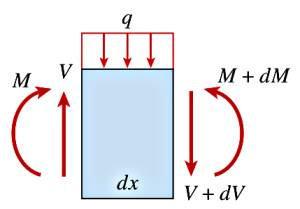
\includegraphics[width=10em]{phy_020_strs_02_10.jpg}

Bu ufak parçanın üzerindeki kuvvetler görülüyor, üstte dağıtık (distributed) bir
yük var, bu bir kesme etkisi $V$ yaratır, ayrıca bükülme momentleri de
mevcuttur. İşaret notasyonu olarak yükler aşağı ise pozitif, moment için
saat yönü tersi pozitif, saat yönü negatif.

Şimdi ilk önce dikey yöndeki kuvvetlere bakalım, burada yük, ve kesme
kuvvetleri var. Üstteki figürde görülen yatay yöndeki tüm kuvvetlerin toplamı
denge gerekliliği sebebiyle sıfır olmalıdır [6, sf. 321].

$$
\sum_{dik} = 0, \quad V - q \ud x - (V + \ud V) = 0
$$

Yani

$$
\frac{\ud V}{\ud x} = -q
\mlabel{3}
$$

Böylece kirişin üzerindeki dağıtık yük ile aynı kiriş üzerindeki kesme
kuvveti arasında bir ilişkiyi ortaya çıkarmış oldum. 

Bükülme Momenti

Momentler için de bir denge formülü ortaya çıkartabilirim. Moment hesabı için
bir nokta seçilmeli, ufak parçanın sağ noktasını baz alıyorum (resimde
işaretli),

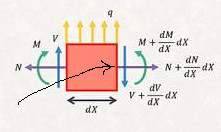
\includegraphics[width=15em]{phy_020_strs_02_11.jpg}

Referans nokta gerekli çünkü hatırlarsak moment bir nokta etrafındaki
döndürmeye bağlıdır, kuvvet dönüş çapına teğet olan kuvvettir. O zaman 

$$
\sum M_{X} = -M + \left( M + \frac{\ud M}{\ud X} \ud X \right) -
V \ud X - q \ud X \left( \frac{\ud X}{2}  \right) = 0
$$

Formüldeki $\ud X / 2$ nereden çıktı? Moment için bir kuvvet uygulama uzaklığı
lazım, uzaklık için de tek bir noktayı seçmek gerekli; bu sebeple $q$'nun etki
ettiği bölgedeki kuvveti tek bir noktaya yapılıyormuş gibi farzediyoruz, o
bölgenin tam ortasına, yani $- \ud X / 2$ noktasına.  Kuvvet büyüklüğü için o
tüm alana etki eden kuvveti bulmak lazım, $q \ud X$.

Devam edelim, $M$ terimleri iptal olur, kalanları tekrar düzenleriz,

$$
V \ud X + \frac{q}{2} \ud X^2 = \frac{\ud M}{\ud X} \ud X
$$

Eşitliğin her yerini $\ud X$'e bölelim,

$$
V + \frac{q}{2} \ud X = \frac{\ud M}{\ud X} 
$$

$\ud X \to 0$ iken limiti alırsak, eşitliğin solundaki ikinci terim yokolur,

$$
V = \frac{\ud M}{\ud X}
\mlabel{4}
$$

Böylece bir eşitlik daha elde ettim, teğetsel / kesme kuvveti $X$'e göre
momentteki değişim oranına eşit. Bir önceki eşitlik yük ve kesme, bu eşitlik
kesme ve moment arasında idi. Bu ilişkiler Statik (Statics) dersinden
geliyor, onları bulmak kolaydı.

Kirişin Yatay Kesme Stresi

Kesme stresi $\tau$'yu bulmak için yine kirişin ufak bir kısmına odaklanalım,

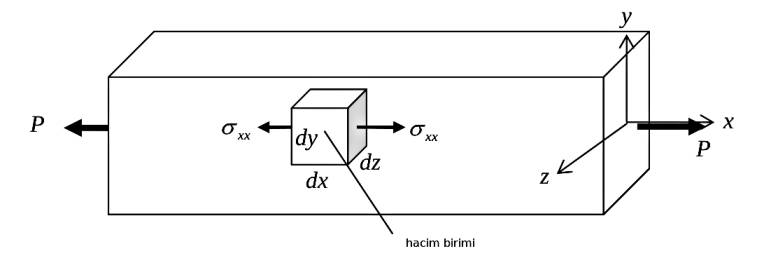
\includegraphics[width=15em]{phy_020_strs_00_06.jpg}

Tüm etki eden kuvvetlerin toplamı sıfır olmak zorundadır [2],

$$
-P + (P + \ud P) + \tau b \ud x = 0
$$

$$
-\ud P/\ud x = \tau b
\mlabel{1}
$$

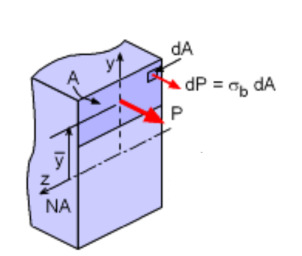
\includegraphics[width=15em]{phy_020_strs_00_01.jpg}

$P$'yi bulmak için $A$ bölgesindeki stresleri entegre ediyoruz,

$$
\int_A \ud P = \int_A \sigma_b \ud A
$$

Fakat daha önce bulduk ki $\sigma_b = -My / I$, yerine koyunca,

$$
P = \int_A - \frac{My}{I} \ud A
$$

$M$ ve $I$ sabittir, entegral dışına çıkartılabilir,

$$
P = - \frac{M}{I} \int_A y \ud A = - \frac{MQ}{I}
$$

Üstte bulunan $P$'yi (4)'e sokunca,

$$
- \frac{\ud}{\ud x} \left( - \frac{MQ}{I} \right) = \tau b
$$

$$
\frac{Q}{I} \frac{\ud M}{\ud x} = \tau b
$$

Şimdi hatırlarsak $\ud M/\ud x$ türevi yatay kesme / teğetsel yükü $V$'ye
eşittir. O zaman

$$
\frac{Q}{I} V = \tau b
$$

Nihai yatay kesme stres denklemi,

$$
\tau = \frac{V Q}{I b}
$$

Kaynaklar

[2] Gramoll, {\em Mechanics},
    \url{http://www.ecourses.ou.edu/cgi-bin/ebook.cgi?topic=me}

[6] Gere, {\em Mechanics of Materials}

\end{document}
